\section{Software stack and design choices}

\begin{figure*}
  \centering
    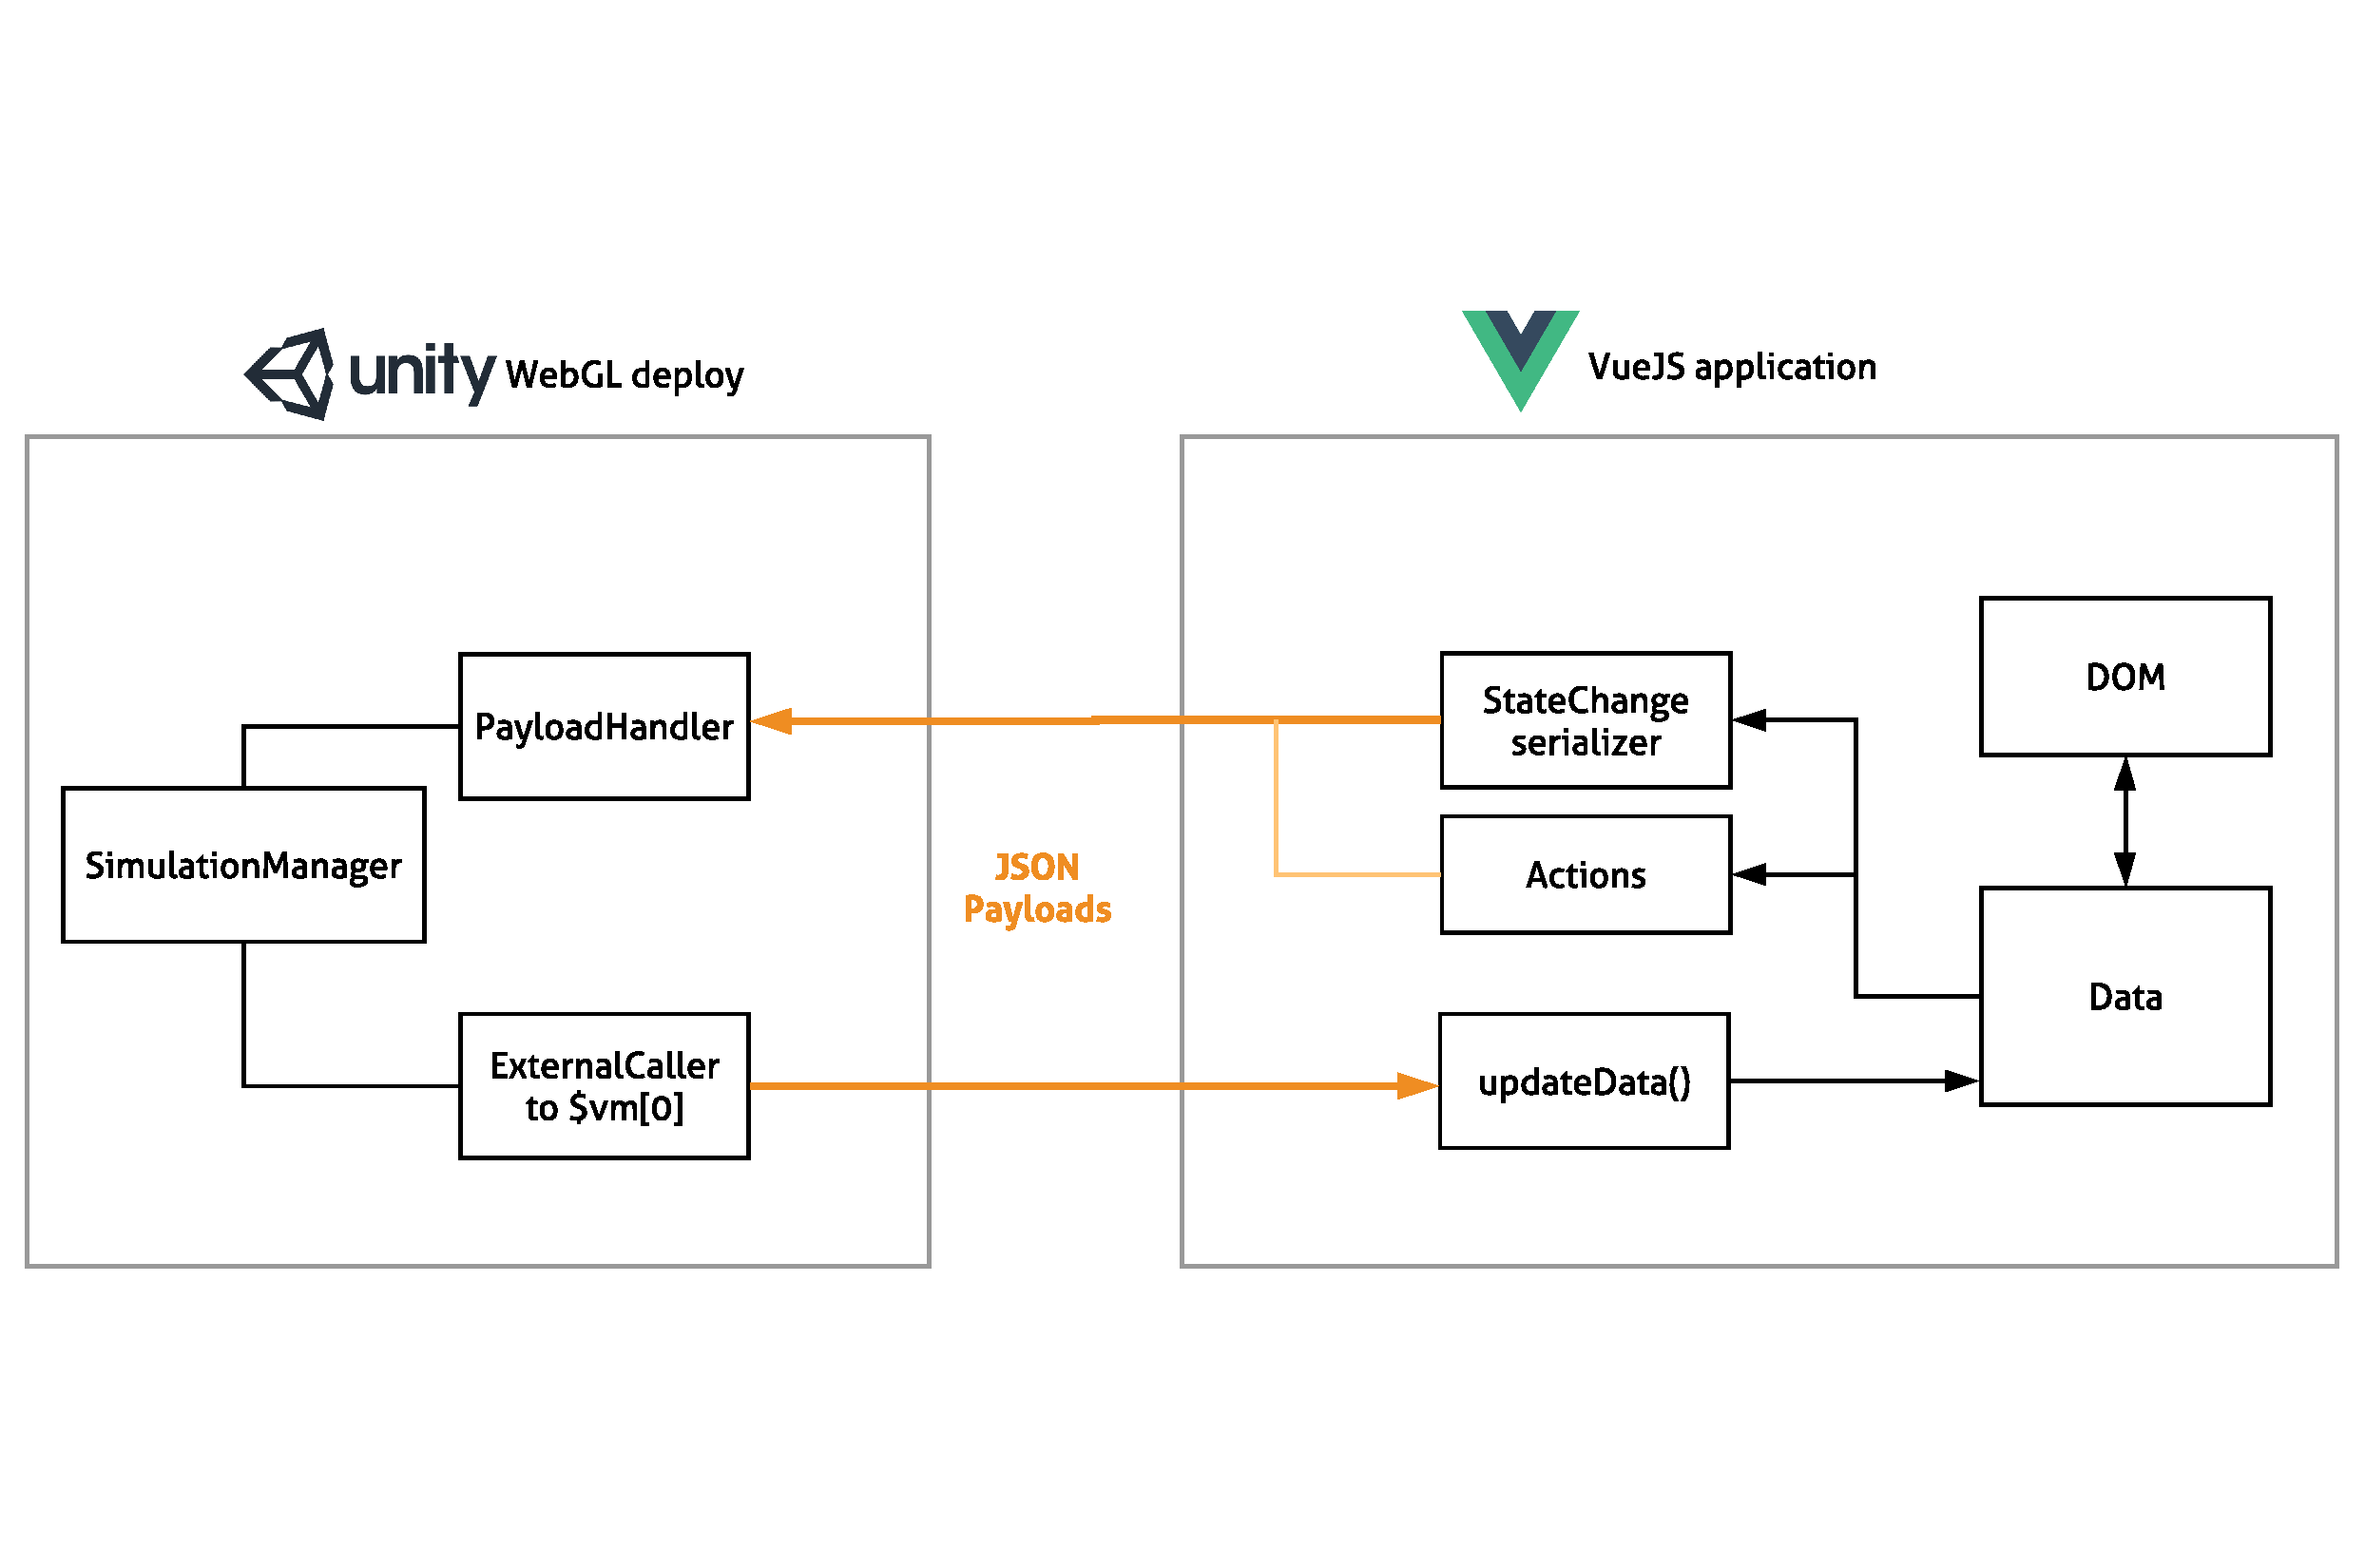
\includegraphics[width=1\textwidth]{sw_arch}%
    
  \caption{Overview of the implemented VueJS - Unity bidirectional comunication}
  \label{fig:swstack1}
\end{figure*}


\section{Simulation framework}


\subsection{Color shading}

One of the most important aspect of the simulation is how to present the results, in real time and in a meaningful and intuitive way. 

We wanted to put focus on one particular feature: the transition of the mass among cells, both on the smaller and the outer range.

This means we needed a smooth animation, making use a changing color tone, representing the steady and consistent movement and formation of the slime mould navigating the map, while expressing how the mass density was changing and moving among areas.

\paragraph{Linear interpolation approach}

The initial approach we considered was a standard linear interpolation: assuming colors are given as triples $(r_1,g_1,b_1)$ and $(r_2,g_2,b_2)$ in the RGB color system, we can fade between them with a simple \textit{linear interpolation}:

\begin{align}
r' &= (1-t)\cdot r_1+t\cdot r_2\\
g' &= (1-t)\cdot g_1+t\cdot g_2\\
b' &= (1-t)\cdot b_1+t\cdot b_2
\end{align}

This gives a blended color $(r',g',b')$ for all $t\in[0,1]$. For $t=0$ it will give the first color, for $t=1$ the second color.


$$ C_1=\begin{pmatrix}r_1\\g_1\\b_1\end{pmatrix}, \qquad C_2=\begin{pmatrix}r_2\\g_2\\b_2\end{pmatrix}$$

The blended color is given as the vector $C'(t)=(1-t)\cdot C_1+t\cdot C_2$.


\begin{figure*}
  \centering
    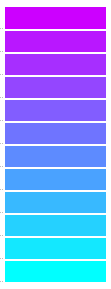
\includegraphics{colorshade1}%
    
  \caption{Color Shading example}
  \label{fig:color}
\end{figure*}


\paragraph{Prescaling and tuning}

The value we want to represent with color is the \textit{Mass} of every single cell. This values varies greatly (and with a different rate based on the model), but we're particularly interested in the growth of smaller values (the mould exploring) and the internal movement of mass.

The different rate of growth is taken into account using two different prescale factors: the mass on the Paper model is reduced by a factor of 50, while ours is reduced by a factor of 10.

We also don't want to represent any value exceeding a threshold since nothing interesting happens after a certain value, and we do not want to focus on something not effecting the actual behaviour of the simulation. This threshold was set to 1000 for the Paper simulation and 100 for the experimental one.

\paragraph{Chosen color shading algorithm}

Following the ideas of the linear interpolation, our color shading algorithms works in the following way. We express colors in Unity's class using RGB triples, with each value in the 0-1 range.\\

PaperModel:

\begin{itemize}
	\item Empty cells are white. C= $(1,1,1)$
	\item Cell mass is scaled with a factor of 50 (40 on low-mass cells). $PM = PM/50$
	\item On low-mass cells ($PM < 15$): C= $(1-PM,1-PM,1)$
	\item C= $(1-PM,PM,3)$
\end{itemize}

Experimental Model:

\begin{itemize}
	\item Empty cells are white.
	\item Cell mass is scaled with a factor of 10. $PM = PM/10$
	\item C= $((0.8-PM)*1.25,(PM-0.20)*1.25,1)$
\end{itemize}

The result is shade of light blue to blue-purple where the lighter values represent more action, more mass and general more mass movement activity, while the darker are the expansion front of the slime mould. The color range is also confined in a precise range (light blue to purple) with offsets on the Red and Green component of the color.

\paragraph{Additional expanding shading for the Paper simulation}

Since the paper simulation is expading extremely fast with a very low amount of mass, each run launched with our color shading algorithm was immediatly flooding the entire map, making the color shading pretty much useless until the mass started to grow near the S points.

So, for the lower values, we chosen to represent the initial expansion with another color shading formula, giving a very subtle (and almost transparent) shade of blue around the front of expansion of the slime mould.

\section{User Interface}
